%% Regular, article-style document with 12pt font and A4 sized paper
\documentclass[12pt,a4paper]{article}

%% UTF-8 support
\usepackage[utf8]{inputenc}

%% Basic packages for formulas, symbols, etc
\usepackage{amsmath}
\usepackage{amsfonts}
\usepackage{amssymb}

%% Use 1 inch margins
\usepackage{fullpage}

%% Hyperlink support
\usepackage{hyperref}

%% Image support
\usepackage{graphicx}

%% For description sections (indentable lists)
\usepackage{enumitem}

%% Custom command to create todo notes. This is a red framed box that contains
%% wrapped, bold, red text.
\usepackage{xcolor}
\newcommand\todonote[1]{\noindent{\color{red}\fbox{\parbox{\dimexpr\linewidth-2\fboxsep-2\fboxrule}{\textit\large{\textbf{TODO: #1}}}}}}

%% Header and footer styles (page number centered at the bottom)
\usepackage{fancyhdr}
\usepackage{lastpage}

%% Makes the tables break over multiple pages. If you don't like this
%% behavior, remove this line and replace all instances of "longtable"
%% with "tabular"
\usepackage{longtable}

%% Don't indent tables (we need every centimeter we can get)
\let\TAB\tabular
\renewcommand\tabular{\noindent\TAB}  

\begin{document}

%% No page numbering until we get to the main section
\pagenumbering{gobble}

%% Title page
\begin{titlepage}
	\vspace*{\fill}
		\begin{center}
			{\huge{\textbf{File Backup and Management System}}} \\
			\bigskip
			{\Large{\textbf{Milestone 6}}} \\
			\bigskip
			\bigskip
			\bigskip
			\bigskip
			{\Large{\textbf{Submitted by: } \\
			Group 06}} \\
			\begin{description}[labelindent=5cm]
				\item Mike Hoffert - mlh374
				\item Syed Ahsan Rizvi - sar457
				\item Hattan Alsharif - haa775
				\item Da Tao - dat293
				\item Michael Butler - mdb815
			\end{description}
			\bigskip
			\bigskip
			\bigskip
			\bigskip
			\Large{\textbf{Date:} \\
			November 23, 2013}
		\end{center}
	\vspace*{\fill}
\end{titlepage}
\clearpage

%% Abstract
\begin{abstract}
The \textit{File Backup or Management System}, henceforth referred to as \textbf{FBMS}, is a system for backing up files while maintaining revisions. FBMS monitors the file operations that take place within the folder that the user wants to backup (called the "live directory"). Not only are file changes copied to the specified backup directory, but revisions (the instance of the file at a given time) are stored in a database, allowing the program to restore the file's state from any point of time. \\

FBMS works on all locally accessible drives, including external drives and network drives. The revisioning creates a patch file for plain text, keeping file size down. For binary files, the entire file is stored as the revision. This revisioning ensures not only are the user's files safe, but erroneous changes can be reverted. \\

FBMS has a focus on ease of use. A wizard guides the user through the setup, where the backup and live directories are chosen. With that complete, the program will run in the background and needs no user interaction until the use desires to restore or view files from the backup.

\todonote{Review and revise}
\end{abstract}
\clearpage

%% Table of contents
\tableofcontents
\setcounter{tocdepth}{3}
\clearpage

%% Page numbering starts here. We begin using the "fancy" page style to allow us to
%% have "page x of y" in the footer. We also have to remove the default headers.
\pagenumbering{arabic}
\pagestyle{fancy}
\fancyhf{} %% Remove the default text
\renewcommand{\headrulewidth}{0pt} %% Remove the header bar
\cfoot{\thepage\ of \pageref{LastPage}} %% New footer content

%% Various content sections. \section denotes level 1 headers, \subsection is level 2,
%% \subsubsection is level 3. All sections automatically added to ToC.
\section{Introduction}

\subsection{System description}
FBMS is an automated backup and revision program. The user specifies a folder that they want to keep backed up (the "live directory") and the location to store the backup (the "backup directory"). The program automatically copies changes in the live directory to the backup directory. Revisions are automatically created by creating "patch" files for every change. \\

Thus, not only is the user's data backed up, but older versions of the data are also backed up. FBMS can be thought of as a hybrid of a local-only Dropbox\cite{dropbox} and a version control system. While it's not as customizable as a version control system like SVN\cite{svn} or git\cite{git}, FBMS is easy to use and runs in the background without the need for user interaction. \\

FBMS backs up and revisions both plain text and binary files. A maximum file size to backup can be set. It's also possible to configure the system to remove revisions older than a certain date.

\subsection{Business case}
FBMS helps ensure the user's files are safely backed up without having to depend on limited cloud-based services or the complexity of programs like SVN\cite{svn}. Programs like Dropbox\cite{dropbox} keep revisions of files, but are limited in their ability to do so. FBMS removes these shackles, limiting you only by your hard drive capacity. FBMS currently supports multiple drive systems, including network drives, filling in the blanks of programs like Dropbox, which are online only.

FBMS differs itself from other backup systems in how it doesn't just backup files, but keeps revisions for safety. FBMS is targeted as the semi-casual audience, who know enough to understand the need for backups, but don't want to use a version control system (or perhaps don't like using such systems). The program is low effort to setup and requires no struggling with command line utilities. Once it's setup, it can run quietly in the background until you need it.

\subsection{User-level goals for the system}
\textbf{A simple to use backup solution for a user's files.}
\begin{enumerate}
\item Ability to back up a folder easily.
\item Iterative backup that allows specific versions to be restored.
\item User can specify any locally available drive (including external and network drives) to serve as the backup or live directory.
\end{enumerate}

\noindent{\textbf{A file versioning and backup solution for their files.}}
\begin{enumerate}
\item User can recover deleted/lost files.
\item User can revert to a prior version of a file.
\item User can view a revision history of the file.
\end{enumerate}

\noindent{\textbf{Gives users a lightweight multi-platform software solution.}}
\begin{enumerate}
\item Able to use this same software on various operating systems due to Java architecture.
\item Once setup, it runs in the background unobtrusively until needed.
\item Tested on Windows, Linux, and Mac.
\end{enumerate}

\subsection{User scenarios}
\textbf{A user wants to backup files:} \\
\noindent{The user will start up the software. The first start wizard will guide the user through setting the live and backup directories. With that done, the system will perform a startup scan, grabbing any files not already in the backup directory. With this done, the software can monitor the file system for changes and act accordingly.} \\

\noindent{\textbf{User has lost the live directory:}} \\
\noindent{User can reinstall the software and specify the existing backup directory. From the GUI, the user can restore the entire backup directory and can set the live directory again.} \\

\noindent{\textbf{User has accidentally deleted a file:}} \\
\noindent{The user can bring up the user interface for our program. They then select the file in question which brings up a list of prior revisions that have been stored. The user can then select the revision they desire to restore and the program will restore it to its directory.} \\

\noindent{\textbf{User wants to minimize file sizes:}} \\
\noindent{The program offers two features to reduce the storage impact of the system. One is to set the maximum file size that is revisioned (defaults to 5 MB). Files larger than this will be backed up, but will not have versions stored. Another is to enable the trim features (disabled by default). Trim will remove all revisions older than a specified number of days. Both of these features are configured in the settings dialog, accessed via the GUI menus.} \\

\subsection{Scope document}
\begin{itemize}
\item A front end GUI for the user to specify files to be watched or restored.
\item File monitoring system that makes notes of changes including creation, deletion and renaming.
\item Database that stores file change history and relevant details about the file.
\item Patch creation and application engine (for handling revisions of text files).
\item Ability to maintain a backup of the latest revision to a designated drive.
\item Ability to restore a file from a specified revision. This includes deleted or renamed files.
\item Option to restore all files from the backup.
\item Ability to revision binary files (the full content of the file is stored).
\item A settings dialog for managing configuration for the program.
\item Ability to change the live and backup directories.
\item Features for removing old revisions and not revisioning up large files.
\end{itemize}

\subsection{Project plan / Rough estimates}
Our plan for our project was to take a concurrent engineering approach with some agile methods, such as SCRUM-like meetings and iterative design. We split the project into stages based on the estimated priority of certain features. For example, the file patching was a high priority feature, since the system revolved that feature. With priority figured out, the project was further subdivided amongst our group members. \\

For the most part, group members worked alone. The assignment of components was made to try and balance familiarity with diversity. We wanted the group members to focus on some areas, allowing them to become proficient at that area. For example, Butler focused on the file change handlers, while Rizvi focused on the GUI. But to prevent the group members from being too specific (and thus blind to the other areas of the project), we also diversified our sections. For example, Butler also worked with the database and Rizvi also worked with the data retriever. \\

We only had initial estimates for version 1.0 of the program, which was our base goal. In that, we estimated approximately 25 hours of work per group member for a total of 125 man hours of work on the project. \\

However, we ended up adding many features to our project that were not originally planned. For example, we had not allocated time for the first run wizard, initially. These extra features caused the actual time spent on the project to well exceed the initial estimate. The rough estimate was a slight overestimate for the initially planned features.

\subsection{User involvement plan}
We designed the system with rational uses in mind. Thus, we are not just the system's creators, but also the system's users. This eliminates the need for a dedicated user. Planning was done both individually and together, collaborating on ideas for both the system's use cases and interior workings. \\

The time used from these users was heavily invested in the planning stage, going through several thousand words of planning. We also used user feedback heavily in revising the project. We made many changes to the project based on user feedback, including better display of errors, a wizard for the first run, and a greater deal of configuration.

\subsection{Low fidelity prototypes}
Our initial prototype was created by editing images of windows. With that, we obtained these early prototype: \\

\noindent{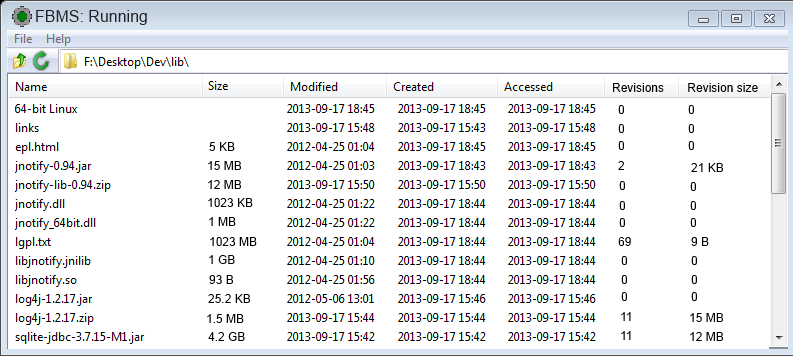
\includegraphics[width=\linewidth]{images/concept.png}} \\

\noindent{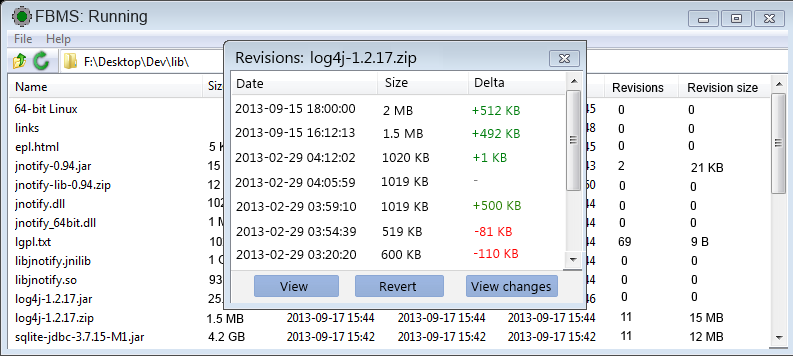
\includegraphics[width=\linewidth]{images/concept2.png}} \\

Our final result is very similar to the mockups: \\

\noindent{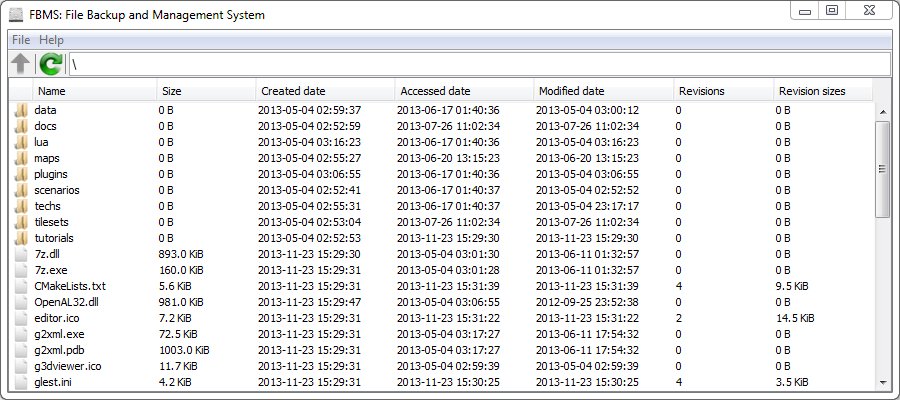
\includegraphics[width=\linewidth]{images/real.png}} \\

\noindent{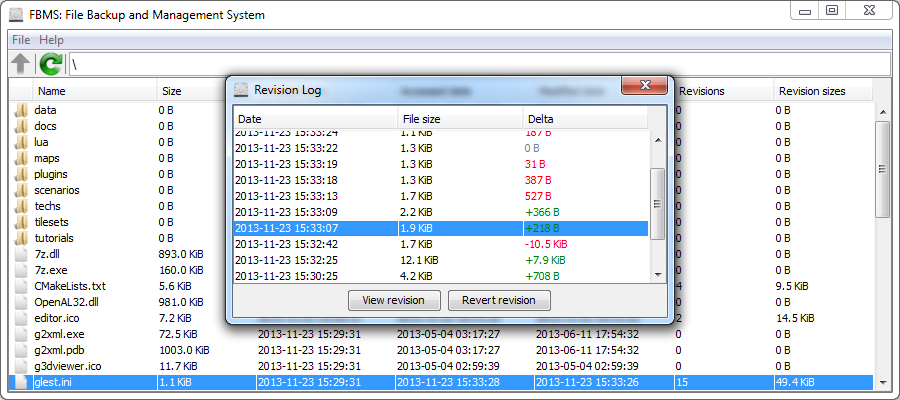
\includegraphics[width=\linewidth]{images/real2.png}}

\todonote{Add linux and mac images of the above cases here (try to get full windows that show off the program well)}

\section{Requirements and early design}

\subsection{Summary use cases}
\textbf{All use cases:}
\begin{itemize}
\item Create file
\item Create folder
\item Modify file
\item Rename file
\item Rename folder
\item Delete file
\item Delete folder
\item Revert revision
\item View revision
\item First run setup
\item Startup
\item Change live directory
\item Change backup directory
\item Change settings
\end{itemize}

\todonote{Need 2 summary use cases per group member. Adapt from M4.}

\subsection{Fully-dressed use cases}
\todonote{Need 1 fully dressed use case per group member. Adapt from M4.}

\subsection{Use case diagram}
\todonote{This one's Da's}

\subsection{Domain model}
\todonote{This one's Michael's}

\subsection{Glossary}
Lorem ipsum dolor sit amet, consectetur adipisicing elit, sed do eiusmod tempor incididunt ut labore et dolore magna aliqua. Ut enim ad minim veniam, quis nostrud exercitation ullamco laboris nisi ut aliquip ex ea commodo consequat. Duis aute irure dolor in reprehenderit in voluptate velit esse cillum dolore eu fugiat nulla pariatur. Excepteur sint occaecat cupidatat non proident, sunt in culpa qui officia deserunt mollit anim id est laborum.

\subsection{Supplementary specification}
Lorem ipsum dolor sit amet, consectetur adipisicing elit, sed do eiusmod tempor incididunt ut labore et dolore magna aliqua. Ut enim ad minim veniam, quis nostrud exercitation ullamco laboris nisi ut aliquip ex ea commodo consequat. Duis aute irure dolor in reprehenderit in voluptate velit esse cillum dolore eu fugiat nulla pariatur. Excepteur sint occaecat cupidatat non proident, sunt in culpa qui officia deserunt mollit anim id est laborum.

\subsection{System sequence diagrams}
Lorem ipsum dolor sit amet, consectetur adipisicing elit, sed do eiusmod tempor incididunt ut labore et dolore magna aliqua. Ut enim ad minim veniam, quis nostrud exercitation ullamco laboris nisi ut aliquip ex ea commodo consequat. Duis aute irure dolor in reprehenderit in voluptate velit esse cillum dolore eu fugiat nulla pariatur. Excepteur sint occaecat cupidatat non proident, sunt in culpa qui officia deserunt mollit anim id est laborum.

\subsection{Operation contracts}
Lorem ipsum dolor sit amet, consectetur adipisicing elit, sed do eiusmod tempor incididunt ut labore et dolore magna aliqua. Ut enim ad minim veniam, quis nostrud exercitation ullamco laboris nisi ut aliquip ex ea commodo consequat. Duis aute irure dolor in reprehenderit in voluptate velit esse cillum dolore eu fugiat nulla pariatur. Excepteur sint occaecat cupidatat non proident, sunt in culpa qui officia deserunt mollit anim id est laborum.

\subsection{Obtaining user feedback}
Lorem ipsum dolor sit amet, consectetur adipisicing elit, sed do eiusmod tempor incididunt ut labore et dolore magna aliqua. Ut enim ad minim veniam, quis nostrud exercitation ullamco laboris nisi ut aliquip ex ea commodo consequat. Duis aute irure dolor in reprehenderit in voluptate velit esse cillum dolore eu fugiat nulla pariatur. Excepteur sint occaecat cupidatat non proident, sunt in culpa qui officia deserunt mollit anim id est laborum.

\section{Updated design and unit testing}

\subsection{System operations}
Lorem ipsum dolor sit amet, consectetur adipisicing elit, sed do eiusmod tempor incididunt ut labore et dolore magna aliqua. Ut enim ad minim veniam, quis nostrud exercitation ullamco laboris nisi ut aliquip ex ea commodo consequat. Duis aute irure dolor in reprehenderit in voluptate velit esse cillum dolore eu fugiat nulla pariatur. Excepteur sint occaecat cupidatat non proident, sunt in culpa qui officia deserunt mollit anim id est laborum.

\subsection{Sequence or communication diagrams with GRASP patterns}
Lorem ipsum dolor sit amet, consectetur adipisicing elit, sed do eiusmod tempor incididunt ut labore et dolore magna aliqua. Ut enim ad minim veniam, quis nostrud exercitation ullamco laboris nisi ut aliquip ex ea commodo consequat. Duis aute irure dolor in reprehenderit in voluptate velit esse cillum dolore eu fugiat nulla pariatur. Excepteur sint occaecat cupidatat non proident, sunt in culpa qui officia deserunt mollit anim id est laborum.

\subsection{Class diagram}
Lorem ipsum dolor sit amet, consectetur adipisicing elit, sed do eiusmod tempor incididunt ut labore et dolore magna aliqua. Ut enim ad minim veniam, quis nostrud exercitation ullamco laboris nisi ut aliquip ex ea commodo consequat. Duis aute irure dolor in reprehenderit in voluptate velit esse cillum dolore eu fugiat nulla pariatur. Excepteur sint occaecat cupidatat non proident, sunt in culpa qui officia deserunt mollit anim id est laborum.

\subsection{Unit testing}
Lorem ipsum dolor sit amet, consectetur adipisicing elit, sed do eiusmod tempor incididunt ut labore et dolore magna aliqua. Ut enim ad minim veniam, quis nostrud exercitation ullamco laboris nisi ut aliquip ex ea commodo consequat. Duis aute irure dolor in reprehenderit in voluptate velit esse cillum dolore eu fugiat nulla pariatur. Excepteur sint occaecat cupidatat non proident, sunt in culpa qui officia deserunt mollit anim id est laborum.

\section{Re-engineering}

\subsection{Code smells}
Lorem ipsum dolor sit amet, consectetur adipisicing elit, sed do eiusmod tempor incididunt ut labore et dolore magna aliqua. Ut enim ad minim veniam, quis nostrud exercitation ullamco laboris nisi ut aliquip ex ea commodo consequat. Duis aute irure dolor in reprehenderit in voluptate velit esse cillum dolore eu fugiat nulla pariatur. Excepteur sint occaecat cupidatat non proident, sunt in culpa qui officia deserunt mollit anim id est laborum. \\

\begin{longtable}{| p{2.75cm} | p{4cm} | p{8cm} |}
  \hline
  \textbf{Clone Pair / Class ID} & \textbf{Root causes} & \textbf{Further comments} \\ \hline
    &  &   \\ \hline
    &  &   \\ \hline
    &  &   \\ \hline
\end{longtable}

\begin{longtable}{| p{2.75cm} | p{12.5cm} |}
  \hline
  \textbf{Clone Pair / Class ID} & \textbf{Why not refactorable / risks in refactoring} \\ \hline
    &   \\ \hline
    &   \\ \hline
    &   \\ \hline
\end{longtable}

\subsection{Refactoring}
Lorem ipsum dolor sit amet, consectetur adipisicing elit, sed do eiusmod tempor incididunt ut labore et dolore magna aliqua. Ut enim ad minim veniam, quis nostrud exercitation ullamco laboris nisi ut aliquip ex ea commodo consequat. Duis aute irure dolor in reprehenderit in voluptate velit esse cillum dolore eu fugiat nulla pariatur. Excepteur sint occaecat cupidatat non proident, sunt in culpa qui officia deserunt mollit anim id est laborum.

\subsection{Gang of Four design patterns}
Lorem ipsum dolor sit amet, consectetur adipisicing elit, sed do eiusmod tempor incididunt ut labore et dolore magna aliqua. Ut enim ad minim veniam, quis nostrud exercitation ullamco laboris nisi ut aliquip ex ea commodo consequat. Duis aute irure dolor in reprehenderit in voluptate velit esse cillum dolore eu fugiat nulla pariatur. Excepteur sint occaecat cupidatat non proident, sunt in culpa qui officia deserunt mollit anim id est laborum.

\section{Complete implementation and product delivery}

\subsection{Naming conventions}
Lorem ipsum dolor sit amet, consectetur adipisicing elit, sed do eiusmod tempor incididunt ut labore et dolore magna aliqua. Ut enim ad minim veniam, quis nostrud exercitation ullamco laboris nisi ut aliquip ex ea commodo consequat. Duis aute irure dolor in reprehenderit in voluptate velit esse cillum dolore eu fugiat nulla pariatur. Excepteur sint occaecat cupidatat non proident, sunt in culpa qui officia deserunt mollit anim id est laborum.

\subsection{Commenting}
Lorem ipsum dolor sit amet, consectetur adipisicing elit, sed do eiusmod tempor incididunt ut labore et dolore magna aliqua. Ut enim ad minim veniam, quis nostrud exercitation ullamco laboris nisi ut aliquip ex ea commodo consequat. Duis aute irure dolor in reprehenderit in voluptate velit esse cillum dolore eu fugiat nulla pariatur. Excepteur sint occaecat cupidatat non proident, sunt in culpa qui officia deserunt mollit anim id est laborum.

\subsection{Pretty-printing of the source}
Lorem ipsum dolor sit amet, consectetur adipisicing elit, sed do eiusmod tempor incididunt ut labore et dolore magna aliqua. Ut enim ad minim veniam, quis nostrud exercitation ullamco laboris nisi ut aliquip ex ea commodo consequat. Duis aute irure dolor in reprehenderit in voluptate velit esse cillum dolore eu fugiat nulla pariatur. Excepteur sint occaecat cupidatat non proident, sunt in culpa qui officia deserunt mollit anim id est laborum.

\subsection{Usability engineering}
Lorem ipsum dolor sit amet, consectetur adipisicing elit, sed do eiusmod tempor incididunt ut labore et dolore magna aliqua. Ut enim ad minim veniam, quis nostrud exercitation ullamco laboris nisi ut aliquip ex ea commodo consequat. Duis aute irure dolor in reprehenderit in voluptate velit esse cillum dolore eu fugiat nulla pariatur. Excepteur sint occaecat cupidatat non proident, sunt in culpa qui officia deserunt mollit anim id est laborum.

\subsection{Complete implementation}
Lorem ipsum dolor sit amet, consectetur adipisicing elit, sed do eiusmod tempor incididunt ut labore et dolore magna aliqua. Ut enim ad minim veniam, quis nostrud exercitation ullamco laboris nisi ut aliquip ex ea commodo consequat. Duis aute irure dolor in reprehenderit in voluptate velit esse cillum dolore eu fugiat nulla pariatur. Excepteur sint occaecat cupidatat non proident, sunt in culpa qui officia deserunt mollit anim id est laborum.

\subsection{User manual}
Lorem ipsum dolor sit amet, consectetur adipisicing elit, sed do eiusmod tempor incididunt ut labore et dolore magna aliqua. Ut enim ad minim veniam, quis nostrud exercitation ullamco laboris nisi ut aliquip ex ea commodo consequat. Duis aute irure dolor in reprehenderit in voluptate velit esse cillum dolore eu fugiat nulla pariatur. Excepteur sint occaecat cupidatat non proident, sunt in culpa qui officia deserunt mollit anim id est laborum.

\section{Project plan, budget justification, and performance evaluation}
Lorem ipsum dolor sit amet, consectetur adipisicing elit, sed do eiusmod tempor incididunt ut labore et dolore magna aliqua. Ut enim ad minim veniam, quis nostrud exercitation ullamco laboris nisi ut aliquip ex ea commodo consequat. Duis aute irure dolor in reprehenderit in voluptate velit esse cillum dolore eu fugiat nulla pariatur. Excepteur sint occaecat cupidatat non proident, sunt in culpa qui officia deserunt mollit anim id est laborum. \\

%% The first column is a tiny little column for the section number.
%% The next column is the actual section name and subsection numbers.
%% Then we have the completed by column. Use \newline to create a new
%% paragraph line inside a table cell.
\begin{longtable}{| p{0.2cm} p{6.25cm} | p{3cm}| p{5cm} |}
  \hline
  \multicolumn{2}{|l|}{\textbf{List of tasks}} & \textbf{Completed by} & \textbf{Comments} \\ \hline
   & Abstract &  &  \\ \hline
  1. & Introduction &  &  \\ \hline
   & 1.1. System description &  &  \\ \hline
   & 1.2. Business case &  &  \\ \hline
   & 1.3. User-level goals &  &  \\ \hline
   & 1.4. User scenarios &  &  \\ \hline
   & 1.5. Scope document &  &  \\ \hline
   & 1.6. Project plan &  &  \\ \hline
   & 1.7. User involvement plan &  &  \\ \hline
   & 1.8. Low fidelity prototypes &  &  \\ \hline
  2. & Requirements and early design &  &  \\ \hline
   & 2.1. Summary use cases &  &  \\ \hline
   & 2.2. Fully-dressed use cases &  &  \\ \hline
   & 2.3. Use case diagram &  &  \\ \hline
   & 2.4. Domain model &  &  \\ \hline
   & 2.5. Glossary &  &  \\ \hline
   & 2.6. Supplementary specification &  &  \\ \hline
   & 2.7. System sequence diagrams &  &  \\ \hline
   & 2.8. Operation contracts &  &  \\ \hline
   & 2.9. Obtaining user feedback &  &  \\ \hline
  3. & Updated design and unit testing &  &  \\ \hline
   & 3.1. System operations &  &  \\ \hline
   & 3.2. Sequence diagrams &  &  \\ \hline
   & 3.3. Class diagram &  &  \\ \hline
   & 3.4. Unit testing &  &  \\ \hline
  4. & Re-engineering &  &  \\ \hline
   & 4.1. Code smells &  &  \\ \hline
   & 4.2. Refactoring &  &  \\ \hline
   & 4.3. Gang of Four design patterns &  &  \\ \hline
  5. & Complete implementation &  &  \\ \hline
   & 5.1. Naming conventions &  &  \\ \hline
   & 5.2. Commenting &  &  \\ \hline
   & 5.3. Pretty-printing &  &  \\ \hline
   & 5.4. Usability engineering &  &  \\ \hline
   & 5.5. Complete implementation &  &  \\ \hline
   & 5.6. User manual &  &  \\ \hline
  6. & Project plan, evaluation &  &  \\ \hline
  7. & Conclusion &  &  \\ \hline
  8. & Acknowledgements &  &  \\ \hline
   & References &  &  \\ \hline
    & \textbf{Total member contributions} & \textbf{Member1} & \\ \cline{3-4}
    &  & \textbf{Member2} & \\ \cline{3-4}
    &  & \textbf{Member3} & \\ \cline{3-4}
    &  & \textbf{Member4} & \\ \cline{3-4}
    &  & \textbf{Member5} & \\ \hline
    & \textbf{Grand total} &  &  \\ \hline
\end{longtable}

%% In this table, the first column is the member name (gonna wanna leave
%% that blank on subsequent rows for a member). Then we have the tasks
%% ("responsible for") column (overriden on the total row). Finally,
%% contributions and comments. This table will probably be cramped, so keep
%% it short and sweet.
\begin{longtable}{| p{4cm} | p{3.5cm} | p{3.5cm}| p{3.5cm} |}
  \hline
  \textbf{Group member} & \textbf{Responsible for} & \textbf{Contributions} & \textbf{Comments} \\ \hline
  Member1 &  &  & \\ \cline{2-4}
   &  &  & \\ \cline{2-4}
   &  &  & \\ \cline{2-4}
   &  &  & \\ \hline
  \multicolumn{2}{|r|}{\textbf{Total for Member1}}  &  & \\ \hline \hline
  Member2 &  &  & \\ \cline{2-4}
   &  &  & \\ \cline{2-4}
   &  &  & \\ \cline{2-4}
   &  &  & \\ \hline
  \multicolumn{2}{|r|}{\textbf{Total for Member2}}  &  & \\ \hline \hline
  Member3 &  &  & \\ \cline{2-4}
   &  &  & \\ \cline{2-4}
   &  &  & \\ \cline{2-4}
   &  &  & \\ \hline
  \multicolumn{2}{|r|}{\textbf{Total for Member3}}  &  & \\ \hline \hline
  Member4 &  &  & \\ \cline{2-4}
   &  &  & \\ \cline{2-4}
   &  &  & \\ \cline{2-4}
   &  &  & \\ \hline
  \multicolumn{2}{|r|}{\textbf{Total for Member4}}  &  & \\ \hline \hline
  Member5 &  &  & \\ \cline{2-4}
   &  &  & \\ \cline{2-4}
   &  &  & \\ \cline{2-4}
   &  &  & \\ \hline
  \multicolumn{2}{|r|}{\textbf{Total for Member5}}  &  & \\ \hline
\end{longtable}

\section{Conclusion}
Lorem ipsum dolor sit amet, consectetur adipisicing elit, sed do eiusmod tempor incididunt ut labore et dolore magna aliqua. Ut enim ad minim veniam, quis nostrud exercitation ullamco laboris nisi ut aliquip ex ea commodo consequat. Duis aute irure dolor in reprehenderit in voluptate velit esse cillum dolore eu fugiat nulla pariatur. Excepteur sint occaecat cupidatat non proident, sunt in culpa qui officia deserunt mollit anim id est laborum.

\section{Acknowledgements}
Lorem ipsum dolor sit amet, consectetur adipisicing elit, sed do eiusmod tempor incididunt ut labore et dolore magna aliqua. Ut enim ad minim veniam, quis nostrud exercitation ullamco laboris nisi ut aliquip ex ea commodo consequat. Duis aute irure dolor in reprehenderit in voluptate velit esse cillum dolore eu fugiat nulla pariatur. Excepteur sint occaecat cupidatat non proident, sunt in culpa qui officia deserunt mollit anim id est laborum.

\begin{thebibliography}{9}

\bibitem{dropbox}
  Dropbox: \url{https://www.dropbox.com/}
  
\bibitem{svn}
  Subversion: \url{https://subversion.apache.org/}

\bibitem{git}
  Git: \url{http://git-scm.com/}


\end{thebibliography}

\end{document}